		% options:
% thesis=B bachelor's thesis
% thesis=M master's thesis
% czech thesis in Czech language
% english thesis in English language
% hidelinks remove colour boxes around hyperlinks

\documentclass[thesis=M,english]{FITthesis}[2012/10/20]


\usepackage{float}
\usepackage{graphicx} %graphics files inclusion

\usepackage{amsmath, kbordermatrix, amssymb} %advanced maths
\usepackage{amsthm} %theorems and lemmas

\usepackage[linesnumbered,lined,boxed]{algorithm2e}
\usepackage{enumitem}
\usepackage{dirtree} %directory tree visualisation
\PassOptionsToPackage{hyphens}{url}\usepackage{hyperref}
\usepackage{listings}
\usepackage{color}
% % list of acronyms
% \usepackage[acronym,nonumberlist,toc,numberedsection=autolabel]{glossaries}
% \iflanguage{czech}{\renewcommand*{\acronymname}{Seznam pou{\v z}it{\' y}ch zkratek}}{}
% \makeglossaries

% % % % % % % % % % % % % % % % % % % % % % % % % % % % % % 
% EDIT THIS
% % % % % % % % % % % % % % % % % % % % % % % % % % % % % % 

\department{Department of Theoretical Computer Science}
\title{Meeting Scheduler}
\authorGN{Luk{\' a}{\v s}} %author's given name/names
\authorFN{Koc} %author's surname
\author{Luk{\' a}{\v s} Koc} %author's name without academic degrees
\authorWithDegrees{Bc. Luk{\' a}{\v s} Koc} %author's name with academic degrees
\supervisor{Ing. Jan Baier}
\acknowledgements{THANKS (remove entirely in case you do not with to thank anyone)}

\abstractEN{Summarize the contents and contribution of your work in a few sentences in English language.}

\abstractCS{V n{\v e}kolika v{\v e}t{\' a}ch shr{\v n}te obsah a p{\v r}{\' i}nos t{\' e}to pr{\' a}ce v {\v c}esk{\' e}m jazyce.}

\placeForDeclarationOfAuthenticity{Prague}
\keywordsCS{teorie grafů, Dijkstrův algoritmus, hledání nejkratší cesty v grafu, paralelizace, zpracování dat, OSM}
\keywordsEN{graph theory, Dijkstra algorithm, single source shortest path, parallel algorithm, data processing, OSM}
\declarationOfAuthenticityOption{1} %select as appropriate, according to the desired license (integer 1-6)

% \website{http://site.example/thesis} %optional thesis URL

%%%%%% Theorem package def
\newtheorem{theorem}{Theorem}
\newtheorem{lemma}{Lemma}
\newtheorem{defin}{Definition}
\renewcommand{\qedsymbol}{$\heartsuit$}
%%%%%% Theorem package def

%%%%%% Math def
\DeclareMathOperator{\atantwo}{atan2}
%%%%%% Math def

\begin{document}
\lstset{language=C++,
		keywordstyle=\color{blue},
        stringstyle=\color{red},
        commentstyle=\color{cyan},
        morecomment=[l][\color{magenta}]{\#},
		tabsize=2,
		basicstyle=\tiny,
		literate={~} {$\sim$}{1},
		literate={->} {$\rightarrow$}{1},
		}
% \newacronym{CVUT}{{\v C}VUT}{{\v C}esk{\' e} vysok{\' e} u{\v c}en{\' i} technick{\' e} v Praze}
% \newacronym{FIT}{FIT}{Fakulta informa{\v c}n{\' i}ch technologi{\' i}}

\setsecnumdepth{part}
\chapter{Introduction}

\section{Motivation}
The 21st century is often titled as the century of data. Usage and gathering data influences our lives on a daily basis. Industry, fashion, society, transportation etc. is transforming under the amount of data gathered and evaluated. 

Growing amount of data are being collected, borders of EU countries are loosening and people are discovering new cultures and jobs in a mare global manner. Most of the time the new location is unknown. Finding meeting locations with colleagues or friends, which may have a limited knowledge about the area too, can turn into a difficult task.

The goal of the thesis is to create an application finding the ideal meeting place for a group of people to save time of everyone involved by applying the knowledge of graph theory, geography and computer science.
Nowadays, computers with multiprocessors or graphic cards are affordable for everyone. Therefore, paralellization of sophisticated applications is becoming highly significant. Knowing that, the application should be designed to utilize possibilities of paralellization.

\section{Geographic information system}
Geographic information systems (GIS) are solving problems which are based on geospatial information. To achieve the goal, special tools are being used such as visualization software, remote sensing and geography tools. Remote sensing tools gain information on specific objects or areas from a distance. Geography tools help to observe and research the environmental changes of the earth and its resources, evolution of society and species. Visualization software, then, displays gathered data as 2D or 3D images \cite{Chen10}.

With a drastic change of modern technologies and enormous amount of data piling up, a new science was born---geographic information science---which is focusing on geographic concepts, applications and systems. The new science opens doors to new problems and issues at a global scale, not easily imaginable a few years ago. 

This thesis uses knowledge gathered through the course of time in geographic information science to map graph theory problems on real life data. Therefore, the developed application belongs to the software category GIS software. 


\section{Problem description}
Within this chapter, first it is necessary to define terms from graph theory, since they are being used regularly throughout the thesis. 
\subsection{Graph theory definitions}

\begin{defin}
A \textbf{graph G} is an ordered pair G = (V, E). Non-empty set V contains
vertices (or nodes) and a set E contains edges. Each edge has either one
or two vertices associated with it, called its endpoints. An edge is said to connect its endpoints.
A graph (without multiple edges) can have up to $n^2$ edges.
\end{defin}

The number of vertices $|V|$ is denoted by $N$ and the number of edges $|E|$ is denoted by $m$ throughout this thesis. 

\begin{defin}
Two vertices are called \textbf{adjacent} if they share a common edge, in which case the common edge is said to join the two vertices. An edge and a vertex on that edge are called \textbf{incident}.
\end{defin}

\begin{defin}
A \textbf{directed simple \textit{graph}} $G$ is a pair $(V, E)$, where $V$ is a finite set of \textit{vertices} and $E \subseteq V \times V$ are the $edges$ of a graph $G$. 
\end{defin}

\begin{defin}
A \textbf{walk} in graph is any sequence of adjacent distinct edges. A \textbf{path} in a graph is a sequence of vertices $v_1, v_2 \dots ,v_k$ such that $(v_i,v_{i+1}) \in E$ for all $1 \leq i < k$.  A path with $v_1 = v_k$ is called a \textbf{cycle}.  The \textbf{length} of a path is the number of edges that it uses.
\end{defin}

\begin{defin}
Let $G = (V, E)$ be a directed graph, whose edges are weighted by the function $f: E \to \mathbb{R}$, associating each edge with the real number called the \textbf{weight}. 
The length of a path is the sum of the weights of its edges. This graph is called \textbf{weighted graph}.  
\end{defin}

In this sense the weights can be reinterpreted as the edge lengths. A cycle whose edges sum to a negative value is a \textit{\textbf{negative cycle}}. 

\begin{defin}
Given a graph G, the \textbf{distance} d(x,y) between two vertices x and y is the length of the shortest path from x to y, considering all possible paths in G from x to y. 
\end{defin}


% We call a graph \textit{sparse}, if $m \in O(n)$. We assume that we are given a layout $L: V \to R^2$ of the graph in the Euclidean plane. For ease of notation, we will identify a node $v \in V$ with its location $L(v) \in R^2$ in the plane.

\subsection{Shortest path problem}
\label{sec:SPP}


The shortest-path problem consists of finding a path of minimum length from a given source $s \in V$ to a given target $t \in V$.
Note that the problem is only well defined for all pairs, if $G$ does not contain negative cycles.
Since our problem is based on real values (distance between two points), negative weights and cycles do not occur in thesis.
If there were negative weights, it would be possible to use Johnson's algorithm \cite{Johnson77} to convert the original weighting function $f: A \to \mathbb{R}$ to a non-negative function $ f': A \to \mathbb{R}^+_0$ in time $O(n_m + n^2 \log n)$, which results in the same shortest paths.

\section{Organisation of the Thesis}
The thesis is structured as follows: First, the Chapter \ref{ch:DA} describes the desired attributes of the data and finding possible data sources. The chapter, further, explains how the data can be stored and processed in order to reduce the number of unnecessary nodes. 

Chapter \ref{ch:DOTA} focuses on the overall design of the application, beginning with the algorithms solving the single source shortest path (SSSP) problem. The main algorithm used for the application is Dijkstra algorithm. In order to decrease the computation time, the possible paralellization of Dijkstra algorithm is further explained. The application also requires a basic user interface, which will be also described in Chapter \ref{ch:DOTA}.

In Chapter \ref{ch:Realisation}, the specific implementation of the application is illustrated. More specifically; how the application is implemented within server and client part, which frameworks were used and additional commentary of the code can be found. 

The results of the application are portrayed in Chapter \ref{ch:Results}. Therefore, the results based on the accuracy and time are compared between parallel and single threaded implementation.
\setsecnumdepth{all}


\chapter{Data Analysis}
\label{ch:DA}

\section{Data fitness}
\label{S1: Good data}
As stated in Koc \cite{Koc14}, a proficient functioning of the application requires appropriate data source. The application needs to work with reliable and (preferably) daily updated data. The area of coverage should not be limiting, so that a high number of people would be able to use it. The data format should be unified in order to make manipulation and management effective. Choosing the correct data format also enables the application to combine different data sources.

To sum up the data are required to follow certain criteria:
\begin{itemize}
	\item up-to-date
	\item verified
	\item human and computer readable
	\item easy-to-use and unified format
	\item freely available
	\item maintained, reliable
\end{itemize}


\section{Data format}
Geographical data exist in various formats depending on type and usage of the data. Data representing the elevation of mountains are preferably stored in a different format compared to data representing the location of a point of interest. 
Most of the existing formats typically fall into two main categories: vector format or raster format. 

% According to Esri's GIS dictionary %TODO cite
Both types offer two different ways to represent spatial data. However, the differences between vector and raster data types are equivalent to those in the graphic design world. The Figure \ref{pic:RasterVector}, which graphically explains how these two types process given data, serves for a better understanding.
%http://i.stack.imgur.com/Y84dG.png

\begin{figure}[h]
\centering
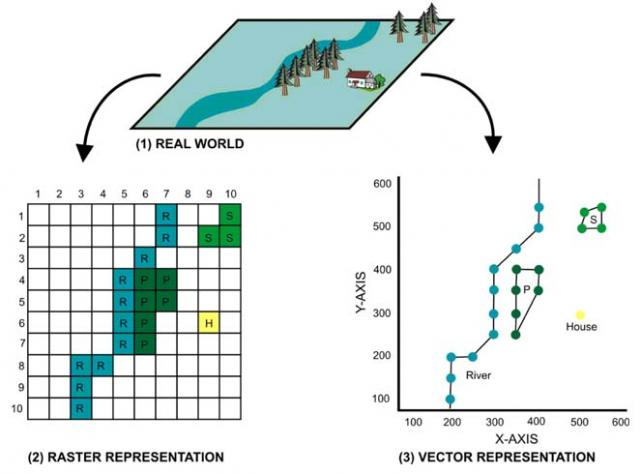
\includegraphics[width=0.8\textwidth]{pics/RasterVectorPreview}
\caption{Realization of raster and vector data representation, obtained from SQL Server Rider \cite{SQL13}}
\label{pic:RasterVector}
\end{figure}

Both, raster and vector representations carry various sets of advantages and disadvantages as well as different definitions. Therefore, these will be described in the following subsections.

% http://data.geocomm.com/helpdesk/formats.html
\subsection{Raster representation}
Raster type formats consist of equally sized cells arranged in rows and columns to construct the representation of space. Individual cells contain an attribute value and location coordinates. Together they create images of points, lines, areas, networks or surfaces.

\paragraph*{Advantages}
\begin{itemize}[noitemsep]
\item Easy and "cheap" to render
\item Represent well both, discrete (urban areas, soil types) and continuous data (elevation)
\item Grid natures provide suitability for mathematical modeling or quantitative analysis
\end{itemize}

\paragraph*{Disadvantages}
\begin{itemize}[noitemsep]
\item Large amount of data
\item Scaling required between layers
\item Possible information loss due to generalization (static cell size)
\item Difficult to establish network linkage
\end{itemize}

\subsection{Vector representation}
Vector type formats uses vertices as a basic unit. A vertex consists of x and y coordinates to determine its position. Using vertices, it is possible to create any shape to describe any object. One vertex creates a point, two can create a line etc. Objects created by vertices may contain additional attributes about the feature they represent.

\paragraph*{Advantages}
\begin{itemize}[noitemsep]
\item Topology nature
\item Compact data structure
\item Easy to maintain
\item Bigger analysis capability
\end{itemize}

\paragraph*{Disadvantages}
\begin{itemize}[noitemsep]
\item For effective analysis, static topology needs to be created
\item Every update requires rebuilding of topology
\item Continuous data is not effectively represented
\end{itemize}

%\section{Summary -- data usage}
%Most of the official European sources (EuroGeographics, EPSON) require filling a form for each download of data. This process could be the bottleneck for the maintenance efforts of the application, because updating the data would take significant amount of time and would require additional functionality. 

%Next very significant part of the choice is the data format. As was said in subsection HERE_ADD_SECTION well 

The idea of the Meeting Scheduler is to create a graph from the data provided to find the closest location. The graph is by definition a topological space. Therefore, the vector representation makes creating graphs more straightforward. The raster representation is by its nature designed to quickly provide graphical overview of the geographical data.

\section{Possible sources}
\label{sec:posSources}

While searching for data, the main focus was not only laid on data in vector type format, but also on sources providing free data of Europe available to the public. In the following subsections are described sources which match these as well as the criteria mentioned in section \ref{S1: Good data}.

%\subsection{Global map data}
%Global map data provided and managed by International Steering Commitee for Global Mapping.
%TODO
 
\subsection{EuroGeographics}
EuroGeographics is the membership association consisting of 60 organizations and 46 countries. It was created in the year 2002, when the Comit{\' e}e Europ{\' e}en des Responsables de la Cartographie Officielle (CERCO) and the Multi-purpose European Ground Related Information Network (MEGRIN) merged together. Its goal is to gather and collect spatial and infrastructural data of Europe \cite{Euro16}. 

EuroGeographics association provides the following products: EuroBoundaryMap, EuroGlobalMap, EuroRegionalMap and EuroDEM.
EuroBoundary map mostly covers borders and administrative informations, EuroDEM map is commonly used for environmental change research or hydrologic modelling \cite{Euro16}.
EuroGlobalMap and EuroRegionalMap consists of many data sets: the administrative boundaries, the water network, the transport network etc. 
In order to download the data it is required to fill up the registration form.

EuroGeographics provides data in following formats

\begin{itemize}
\item Geodatabase
\item Shapefile
\end{itemize}

EuroGeographics yield a reliable source of data, which would be required by our application. Shapefile format can contain geographical data providing an option of additional attributes for the data. However, the registration form which needs to be filled repeatedly, in order to download the data set, would make the data processing to the bottleneck.

\subsection{OpenStreetMaps}
\label{subsec:DA_OSM}
OpenStreetMaps (OSM) is a project officially supported by the OSM Foundation.
OSM was created to build and provide open\footnote{Open data means, that it can be used for any purpose and by anyone as long as the OSM and it's contributors are credited.} geographical data available to everyone.  

The OMS project was inspired by Wikipedia and is working in the same manner: Users are contributing their maps, gps measurements, aerial photographs etc. Since OSM creation in 2004, its community has significantly increased and the data are being updated daily.
OSM provides data in .osm format, which follows XML rules \cite{OSM17}.

In course of time, various projects were created which work with OSM maps.
Thanks to the Mapzen team and their Metro Extract project it is possible to download any major city data in additional two GIS data formats\cite{OSM17}:
\begin{itemize}
\item Geojson
\item Shapefile
\end{itemize}

OSM data are regularly maintained by the community. Documentation to the data is well written, so that any discrepancy within the data set can be easily resolved. The OSM format requires additional parsing in order to operate with the data, since it is not official GIS format. However, projects as Mapzen provide also additional format varieties to choose from \cite{Mapzen17}.

\subsection{EEA}
The European environmental agency (EEA) is an agency of the European Union providing information about the environment for the public. According to their official site \cite{EEA16} it currently consists of 33 member countries.

EEA offers various different data sets, maps and graphs of national designated areas, ecosystem types of Europe, water state and quality, national communications etc \cite{EEA16}.

Depending on the type, these data are provided in the following formats:
\begin{itemize}
\item Excell table
\item CSV
\item Shapefile
\end{itemize} 

Most of the data sets are displayed in interactive maps available on the \href{http://www.eea.europa.eu/data-and-maps}{EEA website}.

After further investigation of the data sets provided by EEA, it seems they are not being updated regularly. In addition, most of the data sets are results of ecological studies or environmental researches (e.g. monitoring $CO_{2}$ or energy consumption)\cite{EEA16}. Since the Meeting Scheduler application requires transportation data sets, the EEA does not provide fitting data.

\subsection{European Observation Network for Territorial Development and Cohesion}
The European Observation Network for Territorial Development and Cohesion (ESPON) 2013 Programme is mainly financed from European Regional Development Fund (ERDF) and its main goal is:

\textit{"Support policy development in relation to the aim of territorial cohesion and a harmonious development of the European territory \ldots "} \cite{ESPON13}

Data are available as soon as users register and accept the Terms \& Conditions. EPSON 2013 data are handled according to ISO 19115 scheme in two formats:

\begin{itemize}
\item XML
\item Excel file
\end{itemize}

Unfortunately, the data provided by ESPON are having the same disadvantages as data provided by EEA in the previous section: maintainability. Our application requires updated data sets in order to accurately compute the optimal meeting place. Investigating the ESPON page further, the ESPON project was separated into two phases in order to analyse and deliver the goal. First phase starting in July 2008 until February 2011 followed by second phase having a lifetime span from February 2011 to December 2014 \cite{ESPON13}. 


The OpenStreetMaps were chosen as a data source, because the data provided are regularly maintained by the community. In addition, the documentation on OSM Wikipage contains all necessary information needed to learn the user how to immediately start working with the data. A Shapefile format was chosen as data format, allowing the application to work with additional attributes if necessary (e.g. street names, type of road etc.).

\section{Storage}
\label{sec:storage}
%TODO
Since the data source and format question is resolved, the next step is to decide the representation of the graph in the memory. During the history of graph theory, four main representations were established and can be chosen from. In the following subsections a closer look on all four options will be taken.

\subsection{Adjacency list}
An adjacency list stores a graph as a list of vertices. Each vertex, then, contains an information about its adjacent vertices in form of a linked list. 
Adjacency lists are easy to implement and use. 
All vertices in a graph are mapped onto an array of pointers referencing to the first node of a linked list. In case a vertex does not have the adjacent vertices, its pointer is set to null. 
An example of an adjacency list for a simple graph can be found in Figure \ref{pic:AdjacencyList} and will be further used as example to also explain further representations. 

\begin{figure}[h]
\centering
\includegraphics[width=0.8\textwidth]{pics/GraphRep}
\caption{Representation of a graph using the method of an adjacency list}
\label{pic:AdjacencyList}
\end{figure}


\subsection{Adjacency matrix}
\label{subsec:AdjMatrix}
An adjacency matrix is defined as matrix of a size $|V(G)| \times |V(G)|$, where $V(G)$ is a set of all vertices in graph $ G $. Values within the matrix depend on the type of graph. Generally, an adjacency matrix for unweighted graph is defined as a $\textbf{A}(G)=[a_{ij}] $, where $a_{ij}$ is the number of edges joining $v_i$ and $v_j$. If the graph is weighted, the values are from the interval $\langle 0, \infty ) $, where $0$ means two vertices are not adjacent and any non-zero value, meaning they are adjacent with an edge cost of that value\cite{Bondy76}. Although, 1 edge at most must exist between every two vertices.
For the graph G, in the example used in Figure \ref{pic:AdjacencyList}, the adjacency matrix $\textbf{A}$ looks as followed:
\[
\textbf{A}(G) =
\kbordermatrix{
 & v_{0} & v_{1} & v_{2} & v_{3} & v_{4} \\
v_{0} & 0 & 1 & 0 & 0 & 1 \\
v_{1} & 0 & 0 & 1 & 1 & 0 \\
v_{2} & 0 & 0 & 0 & 1 & 0 \\
v_{3} & 0 & 0 & 0 & 0 & 0 \\
v_{4} & 0 & 0 & 0 & 1 & 0 	
}
\]
Rows and columns represent vertices of a graph. In the case of matrix $\textbf{A}$, first row and first column represent vertex $0$, second row and column represent vertex $1$ etc. The value in the third row and fourth column means that vertex 2 is adjacent with vertex 3. % As an interesting observation 
It is noticeable that the graph in example $\textbf{A}$ is directed, therefore the adjacency matrix is not symmetric. %TODO possible extent of directed/undirected graphs

\subsection{Incidence matrix}
Incidence matrix is very similar to the adjacency matrix, but instead of showing relations between vertices themselves it represents relations between vertices and edges. Which means, the size of an incidence matrix is $|V(G)| \times |E(G)|$, whereas $V(G)$ is a set of all vertices and $E(G)$ is a set of all edges in graph $ G $. The incidence matrix of graph G is then $\textbf{M}(G) = [m_{ij}]$, where $m_{ij}$ is the number of times (0, 1 or 2 in case of loop) that the vertex $v_i$ and edge $e_j$ are incident\cite{Bondy76}.

An interesting case is the incidence matrix for a directed graph. In that case the sign of the value within matrix $\textbf{M}$ describes the orientation of the edge. Given the edge $e = (x, y)$, then, in the row of vertex $x$ and the corresponding column for edge $e$, the value is positive. In the row of vertex $y$ and the corresponding column for edge $e$, the value is negative.
For the graph G in the example used in Figure \ref{pic:AdjacencyList}, the incidence matrix $\textbf{M}$ looks as followed:

\[
\textbf{M}(G) =
\kbordermatrix{
 & e_{0} & e_{1} & e_{2} & e_{3} & e_{4} & e_5 \\
v_{0} & 1  & 0  & 1  & 0  & 0  & 0 \\
v_{1} & -1 & 1  & 0  & 1  & 0  & 0 \\
v_{2} & 0  & -1 & 0  & 0  & 1  & 0 \\
v_{3} & 0  & 0  & 0  & -1  & -1  & -1 \\
v_{4} & 0  & 0  & -1 & 0  & 0  & 1
}
\]



\subsection{Sparse matrix}
In mathematics, matrices can be divided into two groups: sparse matrices and dense matrices. The definition might sound somehow vague, but sparse matrices are matrices containing huge amount of zero elements. A dense matrix is the exact opposite: containing very few zero elements \cite{Bondy76}. In previous subsections, it is noticeable that each of the matrices (adjacency and incidence) consist of various zero elements and only a few values are actually useful.

The amount of non-zero elements in the adjacency or incidence matrix depends purely on the degree of vertices in the graph. In both types of matrices, each row serves as a vertex and within non-zero values represent edges incident to the vertex. Depending on the graph, which can be directed or undirected, the amount of non-zero elements in adjacency matrices will differ. Incidence matrices do not change their numbers, because they differ only in sign of the value \cite{Bondy76}. 

For undirected graphs, the number of non-zero elements equals to $$ \sum_{v \in V} \textrm{deg(v)} = 2|E| $$ where $E$ is the set of all edges and $V$ the set of all vertices in the graph. 

The same principle applies to the directed graph of incidence matrices. For directed graphs of adjacency matrices, we can observe that the number of non-zero elements depend on the amount of outgoing edges $\Rightarrow$ out-degree, which is 
$$ \sum_{v \in V} \textrm{deg\textsuperscript{--}(v)} = |E| $$ where $E$ is the set of all edges, $V$ is the set of all vertices in a graph and $deg\textsuperscript{--}(v)$ function returns the number of outgoing edges from the vertex $v$ \cite{Bondy76}.

The reason for mentioning sparse matrices in the first place is that there are functions and operations which could be done only with the sparse matrices, providing better memory usage. The main motivation for this section is the storage scheme in which sparse matrix could be stored. The usage of storage schemes enable all the advantages of regular matrix representation with significantly less memory usage since only the non-zero elements are being stored. According to Yousef Saad \cite{Saad03}, the main 3 storage schemes will be discussed. 

The coordinate format belongs to the simplest storage schemes of sparse matrices. The data structure consists of three arrays: 
\begin{itemize}
\item an array containing all the (real or complex) values of the non-zero elements of the original matrix in any order
\item an integer array containing their row indices 
\item an integer array containing their column indices
\end{itemize}
All three arrays are of length $N$, which is the number of non-zero elements \cite{Saad03}.

Taking a closer look at the adjacency $\textbf{A}$ matrix from section \ref{subsec:AdjMatrix}. Clearly this matrix contains less non-zero elements, therefore it is an example of a sparse matrix. Using the coordinate format, matrix $\textbf{A}$ looks the following:

$$
\begin{array}{c}

AA:
\begin{array}{|c|c|c|c|c|c|}
 \hline
 1 & 1 & 1 & 1 & 1 & 1 \\
 \hline
\end{array}
\\ \\
IR:
\begin{array}{|c|c|c|c|c|c|}
 \hline
 0 & 1 & 2 & 0 & 1 & 4 \\
 \hline
\end{array}
\\ \\
IC:
\begin{array}{|c|c|c|c|c|c|}
 \hline
 4 & 2 & 3 & 1 & 3 & 3 \\
 \hline
\end{array}
\end{array}
$$

Array $AA$ stores values of non-zero elements, array $IR$ stores the row index of the corresponding element and array $IC$ stores the column index of the corresponding element. The memory needed for storing the matrix is now only $3N$ instead of the original $N^2$.  The coordinate format excels with it's simplicity and flexibility.

If the elements inside array $AA$ are listed by row, the array $IR$ could be transformed to store instead only indices of the beginning of each row. The size of newly defined array $IR$ is then $n+1$, where $n$ is the number of rows in the original matrix. On the last position ($+1$), the number of non-zero elements within the original matrix is being written. It also may be represented as an address, where the fictional row begins on $n+1$ position. 

Array $\textbf{A}$ would be described by this scheme as the following:

$$
\begin{array}{c}
AA:
\begin{array}{|c|c|c|c|c|c|}
 \hline
 1 & 1 & 1 & 1 & 1 & 1 \\
 \hline
\end{array}
\\ \\
IR:
\begin{array}{|c|c|c|c|c|c|}
 \hline
 0 & 2 & 4 & 5 & 5 & 6 \\
 \hline
\end{array}
\\ \\
IC:
\begin{array}{|c|c|c|c|c|c|}
 \hline
 1 & 4 & 2 & 3 & 3 & 3 \\
 \hline
\end{array}
\end{array}
$$



The transformation of the $IR$ array and listing elements inside $AA$ by row is called Compressed Sparse Row (CSR) format. In scientific computing CSR format is most commonly used for vector-matrix multiplication while having low memory usage.
Through the years, Compressed Sparse Row format developed to a number of variations. 
For example storing columns instead of rows, a new scheme known as Compressed Sparse Column (CSC) format was created \cite{Saad03}.

The last scheme, I would like to point out, is called the Ellpack-Itpack format, which is very popular on vector machines\cite{Saad03}. The Ellpack-Itpack format stores matrices in two 2-dimensional arrays of the same size $n \times N_{mpr}$, where $n$ is the number of rows of the original matrix and $N_{mpr}$ represents the maximum of non-zero elements per row. The first array contains non-zero elements of the original matrix. If the number of non-zero elements is less then the $N_{mpr}$, the rest of the row is filled with zeros. The second array stores the information about the column in which the specific non-zero element is located. For each zero in the first array, any number can be added.

For the given matrix $\textbf{EIF}$:

$$
\begin{array}{c}
\textbf{EIF} = 
\begin{pmatrix}
4 & 0 & 0 & 1 & 0 \\
0 & 0 & 7 & 0 & 9 \\
0 & 2 & 0 & 0 & 0 \\
6 & 0 & 0 & 1 & 0 \\
0 & 0 & 0 & 4 & 3\\
\end{pmatrix}
\end{array}
$$

the Ellpack-Itpack format looks as followed:
 
$$
\begin{array}{lr}
\textbf{AA} = 
\begin{pmatrix}
4 & 1 \\
7 & 9 \\
2 & 0 \\
6 & 1 \\
4 & 3 \\
\end{pmatrix}
\quad \quad
\textbf{IC} = 
\begin{pmatrix}
0 & 3  \\
2 & 4 \\
1 & 0 \\
0 & 3\\
3 & 4 \\
\end{pmatrix}
\end{array}
$$

\subsection{List and matrix comparison}
%Both matrices and list stores equivalent information about the graph. From incidence matrix we can read which two edges share the same vertex (they are incident) and from adjacency matrix which two vertex are connected with an edge. Adjacency list stores for each vertex node edge information in form of linked list which brings two main benefits. 

Adjacency lists in their essence compactly represent existing edges. 
However, this comes at the cost of possible slow lookups of specific edges.
In case of an unordered list, the worst case concerning the lookup time for a specific edge can become O(n) since each list has length equal to the degree of a vertex.
On the other hand, looking up the neighbours of a vertex becomes trivial, and for a sparse or small graph the cost of iterating through the adjacency lists might be negligible.

Adjacency matrices can use more space in order to provide constant lookup times. Since every possible entry exists, it is possible to check for the existence of an edge in constant time using indexes. However, the lookup time for a neighbour becomes O(n) since it is needed to check all possible neighbours.

Data used in the application produce sparse and/or large graphs, for which adjacency list representation is suited better.



\section{Preprocessing}
\label{sec:preprocessing}
Data are being read from Shapefile source obtained via OpenStreetMaps. After further analysis of the Shapefile provided by Mapzen (Section \ref{subsec:DA_OSM}), each data entry is being represented as a line $\Rightarrow$ two nodes sharing an edge. At this point, the edge is missing its weight. Therefore, first step of preprocessing is to weight all the edges within the graph, described in following sections.

\subsection{Great Circle Distance and Harvesine formulae}
\label{subsec:GCD}
The weight of the edge should represent the price of getting from one node into the other. Our application is trying to find the shortest path from multiple sources into one source. Therefore, the price should be based on the distance between source points and the final node, the shorter the better. 

Each node has its specific coordinates $\Rightarrow$ latitude and longitude. This pair represents unique identifier for every node in the application. Let us have two nodes: node $n$ having coordinates $lat1$ and $long1$, and node $m$ having coordinates $lat2$ and $long2$. If $lat1$ = $lat2 \wedge long1 = long2$, then node $n = m$. If $n \neq m$, then at least one of the coordinates differs between nodes $n$ and $m$ meaning the distance between these two nodes is greater than zero.

The simplest solution to compute the distance between two points is using the Pythagorean theorem.

$$
d = \sqrt{(\Delta x)^2 + (\Delta y)^2} = \sqrt{(x_2 - x_1 )^2 + (y_2 - y_1)^2}
$$

where $d$ is a distance between the nodes $(x_1, y_1)$ and $(x_2, y_2)$. If we map latitude on $x$-coordinate and longitude on $y$-coordinate, we would get the distance between two real points, but in a two dimensional space. For computing the distance on Earth, it is needed to use the great circle distances.

The great circle distance takes into account the curvature of the sphere, to provide more precise distance. Using great circle distance allows the application to provide decent approximation between every two nodes (obtained from the data-source) connected via one edge.

To compute the great circle distance on a sphere, the harvesine formula is used: 

$$
\begin{array}{l l}
Harvesine formula: & a = \sin^2(\Delta \psi /2) + \cos \psi_1 \cdot \cos \psi_2 \cdot \sin^2(\Delta \lambda /2) \\
& c = 2 \cdot \atantwo ( \sqrt{a}, \sqrt{1 - a} ) \\
& d = R \cdot c
\end{array}
$$ 

The Meeting Scheduler application is designed to work with the selected data-source (Section \ref{sec:posSources}). The graph is being represented as an adjacency list with weighted edges based on the real life distance. However, most of the world applications work with large amount of data. Therefore, in order to handle big amount of data, it is possible to use either clustering or node reduction, both described in following sections.

\subsection{Graph clustering}
\label{sec:Clustering}
Clustering is a method to group multiple nodes based on similarity into one set -- a cluster. However, in some of the clustering literature, a cluster in a graph is also called a community \cite{Newman04}. An example of clustering is displayed on Figure \ref{pic:Clustering}.


\begin{figure}[h]
\centering
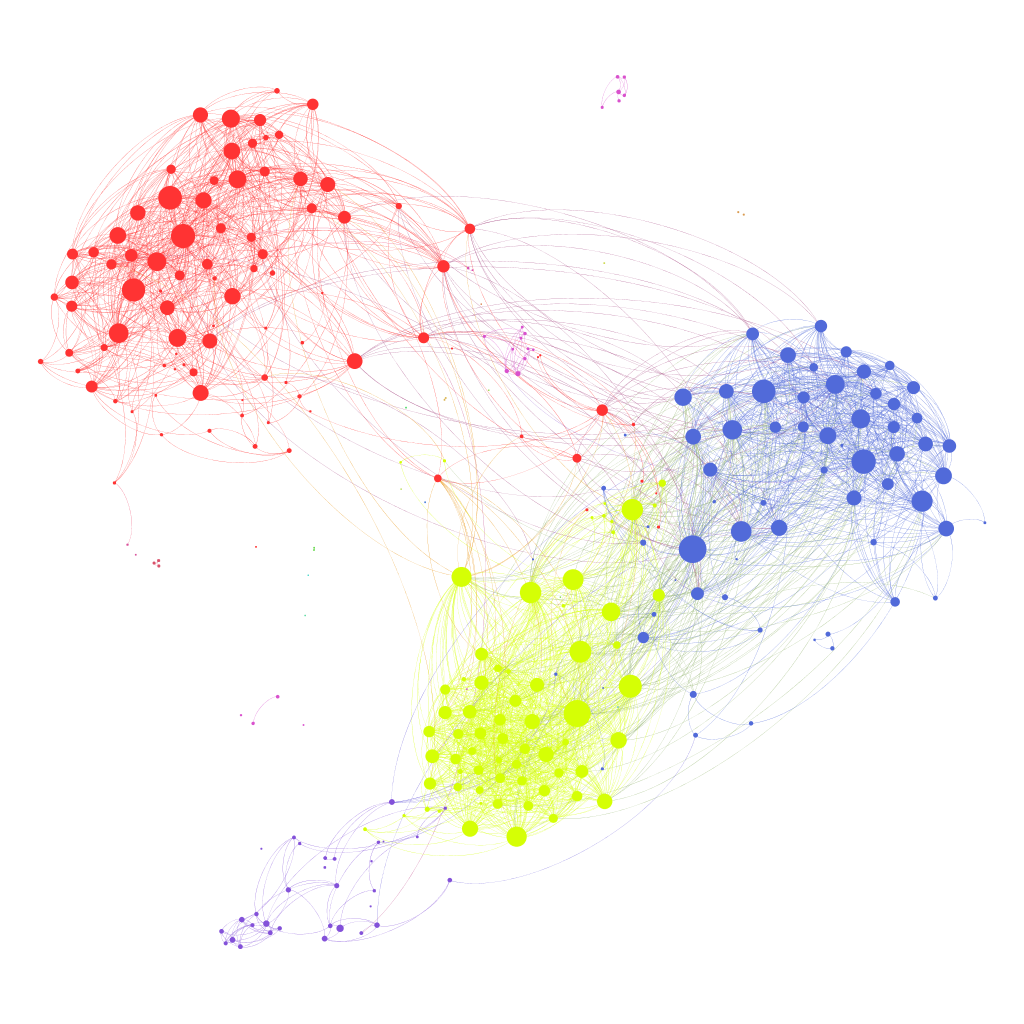
\includegraphics[width=0.8\textwidth]{pics/clustering}
\caption{Clustering applied on the graph of a social network \cite{Griffen17}}
\label{pic:Clustering}
\end{figure}

In survey conducted by S. E. Schaeffer \cite{Schaeffer07}, clustering is formally defined as followed: \textit{``Given a data set, the goal of clustering is to divide the data set into clusters such that the elements assigned to a particular cluster are similar or connected in some predefined sense.''}

The survey further describes two approaches: global clustering and local clustering. In global clustering, every vertex of the input graph is assigned to a cluster, which is the output of the clustering method. However, in the local clustering, only a certain amount of vertices are assigned to clusters. 

The local approach is more suitable for large graphs, since global clustering is computationally demanding for massive data sets. The running time of a clustering algorithm should not grow faster than $O(n)$ in order to be scalable. Local clustering is based on the graph format, which allows access to connected subgraphs or adjacency lists of nearby vertices. Therefore, the clusters can be computed one at a time based on the limited view of the graph topology \cite{Schaeffer07}.




\subsection{Node reduction}
\label{sec:NodeReduction}
The Meeting scheduler transforms real world spacial data into a graph. Spacial data are widely used to map and describe the Earth. In order to be accurately describe any object of the surrounding it is necessary to record every little detail. Figure \ref{pic:Road} displays an example. A road from point A to point B is interpreted as a bended line between two nodes. But in the spacial data it is represented by a group of linked nodes to depict the curvature of the road.

\begin{figure}[H]
\centering
\includegraphics[width=1\textwidth]{pics/road}
\caption{Road on a map represented within the data}
\label{pic:Road}
\end{figure}

For the purpose of finding the optimal meeting place between 2 and more people, it is not required to have all the nodes forming the road saved in the memory. The road on Figure \ref{pic:Road} could be represented only as a pair of nodes, A and B. That way the other 4 nodes representing the road would could be deleted and therefore memory would be conserved. 

The nodes legitimate for removing will be called \textit{connecting} nodes. Within the scope of the thesis connecting node will be defined as following:

\begin{defin}
\label{def:connect}
Connecting node is a node having at most one outgoing edge and at most one incoming edge. 
\end{defin}

It is possible to define transit node in a similar way, which is the opposite of the connecting node. 

\begin{defin}
\label{def:transit}
Transit node is a node having at least two outgoing edges or at least two incoming edges. 
\end{defin}

An examples of a connecting and a transit node is depicted on Figure \ref{pic:CaTnodes}.

\begin{figure}[H]
\centering
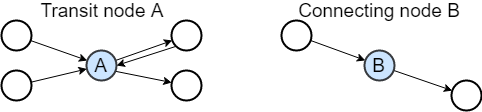
\includegraphics[width=1\textwidth]{pics/CaTNodes}
\caption{An example of a transit and a connecting node.}
\label{pic:CaTnodes}
\end{figure}


Locating and removing connecting nodes from the data source significantly reduce the number of nodes within the graph. However, removing every connecting node would cause the loss of accuracy, because the meeting point would be only located on the intersections or junctions of the roads. It would not be possible to be able to meet in the middle of the street. 
Resolving the dilemma between memory and accuracy highly depends on the given data scenario. The possible solutions are either allowing the user to choose his own precision rate or leaving it up to the developer to decide how the data will be reduced. The solution to the problem used in this application will be further described in the Realization Section \ref{subsec:dataprocessing}.

\chapter{Design of the application}
\label{ch:DOTA}

\section{The shortest path algorithms}
Nowadays, many algorithms exist for solving the shortest path problems exist. Most of them evolved from their predecessors. Each of them solves the problem with different parameters. 
The following list contains the essential algorithms solving the shortest path problem, which lay the foundation in graph theory science:
\begin{itemize}
\item Dijkstra's algorithm
\item Bellman-Ford algorithm
\item Floyd-Warshall algorithm
\item Johnson's algorithm 
\end{itemize}

The Dijkstra's algorithm \cite{Dijkstra59} and the Bellman-Ford algorithm \cite{Bellman58, FordFulkerson62} solve the single-source shortest path (SSSP) problem. SSSP problem can be defined as: Find the cost of the least cost path from $v$ to $\forall w \in V$, given a directed graph $G = (V,E)$ with non-negative costs on each edge and a selected source node $v \in V$. The cost of a path is simply the sum of the costs on the edges traversed by the path. Dijkstra's algorithm is a greedy algorithm working with the graph were negative edges are not allowed \cite{Dijkstra59}. The Bellman-Ford algorithm is a non-greedy version of the Dijkstra's algorithm which allows to work with graphs having negative edges \cite{Bellman58, FordFulkerson62}.

The Floyd-Warshall algorithm \cite{Warshall62, Floyd56} and Johnson's algorithm \cite{Johnson77} solve the all-pair shortest path (APSP) problem. The Floyd-Warshall algorithm iterates all vertices $v$, in order to find a better path for every pair going through $v$ in time $O(N^3)$. Johnson's algorithm, first, converts all the negative edges into positive ones and then, applies Dijsktra's algorithm on every node within the graph. 
For sparse graphs, Johnson's algorithm provides faster computation time than Floyd-Warshall algorithm \cite{Cormen01}.


\section{Dijkstra algorithm}
\label{sec:dijsktra}
The algorithm was conceived by Edsger Wybe Dijkstra in 1956 and was officially published in 1959. Dijkstra's original idea was to find the shortest path between two nodes \cite{Frana10}. However, over the course of time, among computer scientists, Dijkstra algorithm was accepted as an algorithm finding a path from one single node to all other nodes in the graph \cite{Mehlhorn08}. 


The Dijkstra algorithm was constructed to solve the applied problem: How to get from one point to another using the shortest path possible \cite{Frana10}.
The main criteria used to define the shortest path are either time or distance. Both quantities only have positive values. If these criteria are converted into graph theory, all the edges of the graph need to be positive as well.
The data available will only include possitive values, which are the nodes in the graph. Furthermore the graph will represent the geographical map. Therefore, Dijkstra algorithm will be the algorithm of choice for solving SSSP. 

 \subsection{Definition}
There are many variations of Dijkstra algorithm \cite{Mehlhorn08}. Here is a presented variation, in which nodes can be found in three states: $fresh, open $ and $closed$ (Algorithm \ref{algo_dijkstra}). For each node \textbf{n} the function \texttt{dist}(\textbf{n}) represents the distance from the starting node \textbf{s}. For unreachable nodes the value returned by this function will be undefined. Next to the function \texttt{dist}, there is also the function \texttt{prev}(\textbf{n}), which returns the node for the shortest path back to node \textbf{s}.

\begin{algorithm}[H]
\SetKwFunction{Dist}{dist}
\SetKwFunction{Len}{length}
\SetKwFunction{P}{prev}
\SetKwData{Or}{or}
 set the starting node \textbf{s} as \textit{open} and \Dist{\textbf{s}}$ \leftarrow 0$\;
 \For{for each node \textbf{n} different from \textbf{s}}{
  set node \textbf{n} as \textit{fresh}
 }
 \While{$\exists \textbf{u}$ with state open}
 {
  \textbf{u} $\leftarrow$ $open$ node with minimal \Dist{\textbf{u}} \;
  set \textbf{u} state as $closed$	\;
  \ForEach{neighbour \textbf{w} of \textbf{u}}
  {
   \If{\textbf{w} is fresh \Or \Dist{\textbf{w}} $ > $  \Dist{\textbf{u}} $+$ \Len{\textbf{w}, \textbf{u}}}{
	\lIf{\textbf{w} is fresh}{ 
	set \textbf{w} as open}
	\Dist{\textbf{w}} $\leftarrow$ \Dist{\textbf{u}} $+$ \Len{\textbf{w}, \textbf{u}}\;
	\P{\textbf{w}} $\leftarrow \textbf{u}$   
   }
  } 
 }
\caption{Dijkstra algorithm}\label{algo_dijkstra}
\end{algorithm}

On the line number \textbf{6} in Algorithm \ref{algo_dijkstra}, the choice of the node \textbf{u} means choosing \textbf{u} with \texttt{dist}(\textbf{u}) $ \leq $ \texttt{dist}(\textbf{w}), in which \textbf{w} is every other node having the state $open$.

\subsection{Proof of correctness}

In order to prove the algorithm will stop after a finite number of step and its correctness, it is needed to define lemma about states in which nodes can be:

%%%%% LEMMA 1
\begin{lemma}
Nodes can only change state either from "\textit{fresh}" to "\textit{open}" or from "\textit{open}" to "\textit{closed}".
\end{lemma}
%%%%% LEMMA 1

%%%%% PRoof1
\begin{proof}
The only time nodes can change state are on line \textbf{7} and \textbf{10} of Algorithm \ref{algo_dijkstra}.
\end{proof}
%%%%% PRoof1

%%%%% Theorem 2
\begin{theorem}
\label{theorem2}
Dijkstra algorithm will stop computing after at the most \textit{N} steps iterations of while cycle, where N is a number of nodes in graph. 
\end{theorem}
%%%%% Theorem 2

%%%%% Proof 2
\begin{proof}
From the description of the algorithm and previous lemma, it is clear that the set of closed nodes of a cycle will increase with each iteration by one and its size being between 0 and \textit{N}.
\end{proof}
%%%%% Proof 2

%%%%% Theorem 3
\begin{theorem}
Let $A$ be a set of closed nodes. The length of already found path from $v_0$ to $v$ is the length of the shortest path $v_0 v_1 \dots v_k v$, where nodes $v_0, v_1, \dots , v_k$ are in set $A$.
\end{theorem}
%%%%% Theorem 3

%%%%% Proof 3
\begin{proof}
The proof is constructed by induction of numbers of steps executed. The theorem is clearly correct before and after the first step. 

Let $w$ be a node with the state set closed in the last step. Let us consider a node $v$ which is closed.
If $v=w$, then the theorem is trivial. In the opposite case we will show, that there is a shortest path from $v_0$ to $v$ through nodes in set $A$ not containing the node $w$. Set $L$ as length of the path from $v_0$ to $v$ through the nodes in $A$ without $w$. Because in each step we choose the node with the lowest \texttt{dist}(\textbf{u}) and \texttt{dist} of chosen nodes in each step represents a non-decreasing sequence (weight of the edges are positive). Then the length of the path from $v_0$ to $w$ through nodes in $A$ is at least $D$. Because we have chosen $D$ we know, there exists a path from $v_0$ to $v$ through nodes in $A$ which is not using node $w$.

Now let us consider a node $v$ which is not closed. Let $v_0 v_1 \dots v_k v$ be the shortest path from $v_0$ to $v$, where $\forall v_0, v_1, \dots v_k v \in A$. 
If $v_k = w$, then we changed the \texttt{dist} to the length of this path in current step. If $v_k \neq w$ then $v_0 v_1 \dots v_k$ is the shortest path from $v_0$ to $v_k$ through nodes in $A$. Therefore, we can assume that no nodes $v_0, v_1, \dots v_k $ is not $w$ (according to last paragraph). Hence, the length of the path was already set to the correct value before the current step.

Due to the fact, that after the last step the set $A$ contained only the nodes, into which exists a path from node $v_0$, we have proven the correctness of Dijkstra algorithm.
\end{proof}
%%%%% Proof 3

\subsection{Time complexity}
Now from Algorithm \ref{algo_dijkstra}, we can compute the time general complexity of Dijkstra algorithm. Let us assume we use the array in order to store the distances for all the $N$ nodes. As proven in Theorem \ref{theorem2}, the whole algorithm will execute at the most $N$ steps, in each we are choosing the node from the set of \textit{fresh} nodes having size $O(N)$. In each step we also need to check the number of nodes, which are being connected via edges outgoing from the currently checked node. Number of these checks in total is equal to at most $O(E)$, where $E$ is a number of edges in the input graph. To sum up the time complexity, it equals to $O(N^2 + M)$, i.e. $O(N^2)$ since $E$ can be at the most $N^2$.

It is possible to improve this complexity by using heap instead of an array in order to store the distances. In the beginning, the heap will contain $N$ elements and in each step this number will be reduced by one: We find and delete the smallest one in time of $O(\log{N})$ and adjusting the distances of the neighbours, which take $O(E\log{n})$ through all the edges. In total, the time complexity of the algorithm is $O((N+M) \log{N})$. As mentioned in Section \ref{sec:dijsktra} for real life applications, we expect the graph having a form of a sparse graph, meaning for $M << N^2$ the heap version of the algorithm will provide much more better results.


Dijkstra algorithm is very similar to Bellman-Ford algorithm mentioned in subsection \ref{sec:SPP}. The main difference between these algorithms is repetitive checking of the nodes. Once Dijkstra algorithm closes a node, it will never be checked again. Bellman-Fold algorithm goes through each of the nodes and recalculates the path in case negative edges exists in the graph. Because of this extra step, it is slower then Dijkstra, but can detect whether the graph is valid or not.

Dijkstra algorithm computes the shortest paths from one single node to all of the others in the graph. However, the Meeting Scheduler application is searching for an optimal point given multiple input locations instead of a single one. After applying Dijkstra algorithm on every input node, the graph instance now contains the shortest paths for each input node. Therefore, every node in the graph holds an information about the distance to each of the input nodes. Within these nodes exists one node, having the optimal combination of the shortest paths, which is the result at the Meeting Scheduler application.
This whole computation process leaves a lot of space for the performance optimization, especially the parallelization. 
\newpage
\section{Parallelization of Dijkstra algorithm}
The development of information technology together with the wide range of attention in graph theory research, a variety of algorithms and graph structures have been proposed \cite{Peng09}. Nowadays, the algorithms for serial SSSP optimization have reached the time limitation. The only solution to improve the performance efficiently lies in parallel computation. 

N. Jasika et al.\cite{Jasika12} measured the performances of two implementations of Dijkstra algorithm. One was executed on dual-core processor i5 with OpenMP and second with OpenCL. The measurement of the performances were not as fast as expected. Among possible reasons mentioned were the code, which was not efficient enough, and the input data set, which was small enough. Therefore, more time was spend on synchronization instead of parallel computation.

Two major issues inherent to Dijkstra algorithm were pointed out in the article: limited explicit parallelism and excessive synchronization. Therefore, Dijkstra algorithm represent a challenging example of an algorithm, which is difficult to accelerate. Mainly because it relies on priority queue (see Section \ref{sec:dijsktra}).

The case study made by P. Bogdan \cite{Bogdan15} focuses as well on creating a parallel application using Dijkstra algorithm with a high degree of efficiency. The study proposes that Dijkstra algorithm is very useful in cases of a high density of nodes. Therefore, the algorithm is one of the first steps towards improving the systems in fields such as computer networks, GPS systems or node localization in 3D wireless sensor networks.

Parallelization of Dijkstra algorithm represents one of the toughest parallel problems in graph theory. The key to provide better performances is to identify blocks of code possible for parallelization. The identification of the parallel blocks and solutions is described in the Section \ref{sec:real_parallelization}.

\section{User interface design}
\label{sec:UIDesign}
The application requires the spacial information as input. 
Further, the user should be able to insert the positions of people in order to find a meeting point, which is approximately of the same distance to all positions. For that, the user interface (UI) of the application should provide a way to register and store spacial information provided by the users. 

Creating a fully satisfiable graphical user interface (GUI) is not main purpose of this thesis. So it was decided to create a simple GUI in which users can insert the geographical coordinates of participants. As a result, a single pair of coordinates of final destination will be received. 

A fully optimal GUI would allow users to select a position through the displayed map of the data set available. Finding exact coordinates would be further transcribed into a marked point on the map and the general user-flow would be significantly improved, because the user would see a marked point on the map which would be the meeting point. Example of a fully optimal GUI is displayed in Figure \ref{fig:OptUI}.


\begin{figure}[H]
\centering
\includegraphics[resolution=125]{pics/OptimalUI}
\caption{Design of a fully optimal user interface.}
\label{fig:OptUI}
\end{figure}

The goal of the thesis is to create suboptimal user interface. First, the interface should provide the way to connect to the server, so the communication between server and client could be established. Further, there are several input boxes allowing the user to insert the position of the people. Last, the interface provides the user current status of the application through the logging service. Not only to deliver the result, but also to inform the user about the whole process, for example whether the data inserted are incorrect or the connection has been lost.
Creating suboptimal user interface is described in the next chapter in Section \ref{sec:RClient}.

\chapter{Realisation}
\label{ch:Realisation}

\section{Technology used}
\label{sec:TechUsed}
The goal of the thesis is to create a complex desktop application with a basic front-end to provide users with proper control over the input data and the general overview of the application. In addition, the technology used should be cross-platform. In general, modern high-level programming languages prefer one platform over the other (C\texttt{\#} Windows, ObjC iOS etc.). However, to satisfy as many users as possible usage in all platforms is desired.

In direction of keeping the application as simple as possible, the main computation part of the application is written in C\texttt{++} language, which provides great computing performances on any platform while offering OOP principles in order to create more complex applications. In addition, C\texttt{++} based back-end will make the deployment on any server operating system effortless. Not to mention there are plenty open source libraries available, making a realization of the whole project easily done.  

%% QT 
One of the external tools used for the purpose of the application is Qt framework. Qt provides cross-platform tools to create basic GUI and is classified as FOSS\footnote{Free and open-source software} computer software. Therefore, fitting the purpose of the application being open source. 
Usage of classes and functions of Qt framework is very straightforward while producing fully functional GUI as a front end for the application\cite{QT17}. 

%% GDAL
For reading the data files and following manipulation, GDAL/ORG library was selected. GDAL is designed to read and write raster GIS formats. GDAL library is developed under Open Source Geospatial Foundation and released under the X/MIT license\cite{GDAL17}. 
As an addition to the GDAL is the ORG library which enables usage of simple features for vector formats. Together the whole GDAL/ORG library supports most of the GIS formats \cite{GDAL117}. %cite "GDAL Raster Formats". GDAL - Geospatial Data Abstraction Library. 2011-06-05.	
Since the data set of the application is in Shapefile format (see Section \ref{sec:posSources}), GDAL/ORG library provides optimal tools for reading and collecting information from our data set.

\section{Server}
\label{sec:server}
The Meeting Scheduler application is structured as a server-client model using TCP protocol. As defined in the Linux information project \cite{TCP17}:  \textit{``TCP uses error correction and data stream control techniques to ensure that packets to arrive at their intended destinations uncorrupted and in the correct sequence, thereby making the point-to-point connection virtually error-free.''} 

This feature is expensive, when the amount of data is constant and large (e.g. file transfer). For data streaming is more appropriate user datagram protocol (UDP) \cite{Kurose10}.
However, the Meeting scheduler server and client communicate with using only small sized messages in form of coordinates, therefore the TCP provide optimal solution. 

The \textit{Server} class implementation in Listing \ref{lst:Server} is straightforward and self-explanatory, providing methods to establish connection between client and server and allow further communication.

\begin{lstlisting}[frame=single, caption={\texttt{Server} class}, label={lst:Server}]
class Server
{
private:
    int sock, sockclient;
	struct sockaddr_in serv_addr, cli_addr;
    char buffer[512];
public:
    Server(int );
    int Listen();
    int ReadFromClient(char *);
    int WriteToClient(std::string );
    void CloseClientSocket();
    ~Server();
};
\end{lstlisting}

Server is responsible for providing client the results of their requests, more specifically meeting point based on input received. To achieve that, server should be having data set available and preprocessed, so that computation can start without any delay. Hence, server is split into two parts: data processing module and computation module.

Data processing module is the part of the server ensuring the data are transformed in the corresponding directed graph. The graph will further be provided to another part of the server -- computation module. Both modules are further described in the following sections.


\subsection{Data processing module}
\label{subsec:dataprocessing} 
The role of the data processing module is to transform gathered data sets into directed graph. The data set is represented with the specific GIS file format, more specifically Shapefile format provided by team Mapzen (see Section \ref{subsec:DA_OSM}). The data set obtained has already been partially processed, so it contains only features describing transportation (e.g. road or rails). The data processing module is able to read the selected format and extract all the nodes from the transport points. These nodes represents vertices in the graph. 

Afterwards, the edges are extracted from the relations of the nodes. In addition, each edge obtains the cost based on the great circle distance (see Section \ref{subsec:GCD}) between the points. Together with vertices the full graph is complete.

Based on the size of the graph, the amount of nodes can be reduced using node reduction or the structure of the graph can be modified by clustering. Both methods are described in Section \ref{sec:preprocessing}. These changes to the graph obtained are shortening the computation time for the cost of accuracy. 

The following subsection describes the implementation of the data-reader class, allowing to read and further manipulate the data, e.g. transforming the data into the graph structure. This class represent essential step in data processing module.

\subsubsection{Data-reader class}
%TODO FITNESS, STORAGE, Source
The application is reading data through the class called \texttt{DataReader}. The structure of the class is displayed in Listing \ref{lst:DataReader}. The constructor requires the string, which is representing the path to the Shapefile data-file. Within the constructor the GDAL library opens the file and set the pointer \texttt{GDALDataset * pDS} to the data set within the input file.

\begin{lstlisting}[frame=single, caption={\texttt{DataReader} class}, label={lst:DataReader}]
class DataReader
{
private:
    GDALDataset * pDS;
    OGRLayer * pLayer;
    int featureCount;

public:
    DataReader(std::string );
    int InitLayer(int);
    NodePair GetNodesFromCurrentFeature() const;
    int GetLayerSize() const;
    double static DistanceBetweenTwoPoints(Node * , Node * );
    ~DataReader();
};
\end{lstlisting}

Having the data set initialized, the next step is to load the features within. Features are conained within the layers. Calling the method \texttt{InitLayer(int)}, the layer is initialised, seting the pointer \texttt{pLayer} to the first feature available. The argument of the function determines the index of the layer, if the data set contains more layers. \texttt{OGRFeature} is a container holding a geometry and the attributes of the feature. Geometry types are displayed on the Figure \ref{pic:OGRGeo}, obtained from official GDAL documentation \cite{GDAL17}. 



After analysis of the data set, the geometry of the road is represented as a \texttt{OGRLineString} class. Therefore, every feature contains two nodes connected together via an edge. Method\texttt{GetNodesFromCurrentFeature()} reads the first feature within the layer and returns a pair of nodes connected via edge in form of \texttt{NodePair} structure. \texttt{NodePair} structure contains two pointers to the \texttt{Node} class. 

The last method within \texttt{DataReader} class to point out is the static function\texttt{DistanceBetweenTwoPoints(Node*,Node*)}. The method takes two nodes as arguments and returns the great circle distance between them. It is static since it is not needed to be dependent on any object of the \texttt{DataReader} class.

\begin{lstlisting}[frame=single, caption={\texttt{Node} class}, label={lst:Node}]
class Node{
private:
    double lat;
    double lon;
    Node ** adjNodes;
    double * edgeW;
    int adjNodesCount;
    int maxAdjNodes;
public:
    Node( double, double);
    std::pair<double, double> GetCoords() const;
    double GetLat() const;
    double GetLon() const;
    int GetEdgesCount() const;
    Node ** GetEdges();
    std::pair<Node *, double> GetNode(int ) const; 
	int AddNeighbour(Node * , double );
    ~Node();
\end{lstlisting}

The class \texttt{Node} represents the vertex in the graph and its structure is shown on Listing \ref{lst:Node}. It stores the information about its position and weighted edges to other adjacent vertices. \texttt{Node} forms a foundation for the graph represented as \texttt{Graph} class, shown in Listing \ref{lst:Graph}.

\begin{lstlisting}[frame=single, caption={\texttt{Graph} class}, label={lst:Graph}, breaklines=true]
class Graph
{
private:
    std::map<std::pair<double, double>, Node * > Nodes;
public:
    Graph();
    int AddNodePair(Node *, Node * );
    Node * GetNode(std::pair<double, double>);
    int ConstructGraph(DataReader *);
    int GetSize() const;
    Node * FindClosest(std::pair<double, double>);
    std::map<std::pair<double, double>, double * > CreateDistArray(int);
    static void RemoveDistArray(std::map<std::pair<double, double>, double *> &);
    ~Graph();
};
\end{lstlisting}

\texttt{Graph} is storing nodes in the STL map structure, mapping the coordinates to a specific node. That causes each node to be stored once at the most. The class is constructed with \texttt{ConstructGraph(DataReader *)} using the \texttt{DataReader} as an argument. Within this method, the data set is being read, every feature is being analysed and saved in form of the graph into \texttt{map<pair<double, double>, Node * > Nodes}.

Another noticeable method is \texttt{FindClosest(pair<double, double>)}. It is used to locate the closest node to the specific location. This method is required in order to locate the input of the user in the graph. Again, the method is using great circle distance to find the closest node to the input. 
On the other hand, it is needed to go through the whole graph and measure the distances for each node. 
This leaves the room for optimization of the application.

Except of the generic support methods, there are methods called \texttt{CreateDistArray(int)} and \texttt{RemoveDistArray(map<pair<double, double> > *}. Distance array represents the structure, in which the results of the Dijkstra algorithm are stored. It is a map, mapping the coordinates to the array of distance values. The size of the array is equal to the number of user inputs. Therefore, the distance array stores for every input the distance to every node in the graph. 
\texttt{RemoveDistArray(..)} method serves as a destructor for distance array.

The distance array is being used as a argument for the Dijkstra algorithm, further described in Section \ref{subsec:server_comp}. After storing all the results for each input node, the last step is to go through all the vertices within array and select the one with the shortest distances to each input node.


\subsection{Computation module}
\label{subsec:server_comp}
The computation module uses the graph constructed by the data processing module. Data processing is needed only at the start of the server or after updating the data set. Thereafter, the server waits in stand-by mode, expecting the client to send the input coordinates. Next subsection describes the algorithm, which initiates immediately after establishing the connection with the client and transferring the input data from the user.


\subsubsection{Algorithm}
After receiving the input coordinates from the client, the application is ready to start the computation. 
The main computation algorithm is Dijkstra algorithm (see Section \ref{sec:dijsktra}). Dijkstra algorithm is solving SSSP problem. The application is using Dijkstra algorithm for each of the input nodes, resulting in the shortest distances to all nodes in the graph and choosing the most suitable one.

The version of sequential Dijkstra algorithm uses a priority queue based on the distance to process every node in the graph. A priority queue affects the computation time of the algorithm based on the structure of priority queue \cite{Chen07}. 

The priority queue needs to have following operations, in order to be useful for an algorithm:
\begin{description}

\item[ExtractMin] to get a vertex with a minimum distance for all the vertices, whose shortest distance is not yet found
\item[DecreaseKey] to update the distance of adjacent vertices of currently	extracted vertex; If the distance is smaller than currently found optimum, update the information in the queue

\end{description}

The operations above are guaranteed by \textit{Set} container in C\texttt{++} STL. \textit{Set} keeps all its keys in sorted order \cite{STL17}. Hence, a minimum distant vertex will always be at the beginning, allowing to extract the vertex with the minimum distance (\textbf{ExtractMin}) and update the distances of all other adjacent vertices accordingly (\textbf{DecreaseKey}) $\Rightarrow$ if any vertex's distance become smaller, delete its previous entry and insert new updated entry.

The implementation of the sequential Dijkstra algorithm is located in Listing \ref{lst:SeqDijkstra}. The method has three arguments. The first argument \texttt{g} represent the graph storing all the information about the nodes. The second argument \texttt{source} is a pair of coordinates defining the input node. The third argument \texttt{dist} is a container, storing the distances from every input node to every other node in the graph. The last argument is an index of the input node.

\begin{lstlisting}[frame=single, caption={Sequential Dijkstra algorithm}, label={lst:SeqDijkstra}, breaklines=true]
void MeetingScheduler::SequentialDijkstra(Graph * g , 
		std::pair<double, double> source, 
		std::map<std::pair<double , double>, double * > & dist, 
		int input_index)
{
    // init priority queue based on the distance
    set< pair< double, PD > > pq;

    // insert first node to the queue
    pq.insert(make_pair( 0, source ));
    dist[source][input_index] = 0;


    while (!pq.empty()) {
        // ExtarctMin from the queue
        pair< double, PD> tmp = *(pq.begin());
        pq.erase(pq.begin());
        PD u = tmp.second;
        Node * n = g->GetNode(u);

        // iterate trough the adjacent nodes
        for (int i = 0; i < n->GetEdgesCount(); i++) {
            pair<Node*, double> node_edge = n->GetNode(i);
            double dist_temp  = dist[u][input_index] + node_edge.second;
            if (dist[node_edge.first->GetCoords()][input_index] > dist_temp)
            {
                // 	removing already existing entry from the set; 
                //	for finalized nodes this step is unreacheable
                if(dist[node_edge.first->GetCoords()][input_index]!=DBL_MAX)
                {
                    pq.erase(pq.find(make_pair(
                    	dist[node_edge.first->GetCoords()][input_index], 
                    	node_edge.first->GetCoords())));
                }

                dist[node_edge.first->GetCoords()][input_index] = dist_temp;
                pq.insert(make_pair(
                	dist[node_edge.first->GetCoords()][input_index], 
                	node_edge.first->GetCoords()));
            }
        }
    }
}
\end{lstlisting}

Time complexity depends on the structure used in \textit{Set} container. According to SGI documentation \cite{STL17}, all the \textit{Set} operations (e.g. insert, delete) take logarithmic time. Therefore, the solution in Listing \ref{lst:SeqDijkstra} is $O(E \log V)$.

The method depicted in Listing \ref{lst:SeqDijkstra} is called for each input node, the server receives from the client. The result of each is stored within one structure -- \texttt{dist}. When Dijkstra algorithm finished computing the distances for every input, the next step is to find the node with the best combination of distances.

\subsubsection{Finding the result}

As described in the previous section, each node has the information of the shortest distance to all input nodes. The optimal node needs to have the shortest and uniform distance from every input node. Therefore, the summation and standard deviation is computed for every node. 

The node with the shortest distances to every input node needs to have the smallest summation of all distances. The standard deviation of all the distances achieve uniformity. Therefore, every person has a relatively equal distance to the meeting place (based on the value of the standard deviation). 

The standard deviation (represented as a Greek letter $\sigma$) in statistics measures the amount of variation or dispersion of a set of data values \cite{Bland96}. The smaller the value of the standard deviation is, the more similar the values are. Choosing the result with the smallest standard deviation ensures the uniformity of the result.
The formula used to compute discrete standard deviation for the node $v$ looks as follows:
$$
	\sigma_v = \sqrt{\frac{1}{N} \sum_{i=1}^{N} (x_i - \overline{x})^2}
$$
where $N$ is the amount of input nodes,  $x_i$ is distance from the input at index $i$ to the node $v$ and $\overline{x}$ is mean value of all the distances to the node $v$. 

The optimal node needs to have the smallest summation and standard deviation of all the distances. With growing summation of distances, the fitness of the node is less desired. The same applies to the standard deviation of the distances. Hence, it is possible to put the summation and standard deviation into the relation, creating the fitness value. Therefore, the fitness value of the node is represented as a multiplication of those two values. The node with the smallest fitness value is the optimal node. 

\subsubsection{Analysis of the fitness}
In previous paragraph the fitness value of the node as a multiplication of summation and standard deviation was defined. Since the distance values are within $[0, \infty)$ interval, the summation of them can be within $[0, \infty)$ interval as well. If the summation of the distances is $0$, all of the distances are also $0$. That means all the input nodes are located in the same location. This edge case is already handled in the UI layer of the application, therefore, the summation is within the interval $(0, \infty)$.

The standard deviation is in general (as well as the summation) from $[0, \infty)$. If standard deviation equals $0$, it means all the values are the same. Ideally, the optimal node should have a standard deviation of the distances equal to $0$. However, this fact can completely override the contribution of the summation in the fitness value. Using real world data, it is possible that input nodes have equal distances to multiple nodes, but with different values \footnote{with increasing number of input nodes the probability of having $\sigma$ decreases}. In Figure \ref{fig:TInodes} shows such example for two input nodes.



\begin{figure}[H]
\centering
\includegraphics[resolution=100]{pics/TInodes}
\caption{Example on two possible result nodes for nodes A and B, based purely on smallest value of standard deviation. Node in the middle is having smaller summation of the distances, therefore being the optimal result.}
\label{fig:TInodes}
\end{figure}


There is a special handling of this case, if the standard deviation equals zero. During the processing of all the nodes the summation of the currently optimal node is stored. If another node with the same fitness is found, node with the smaller summation is chosen as the optimal node. 


\subsubsection{Parallelization}
\label{sec:real_parallelization}

\section{Client}
\label{sec:RClient}
The client provides basic GUI for the user. The user thought the client connects to the remote server and send the server locations of people.
The appearance of the current UI was created by Qt framework as mentioned in the beginning of the Section \ref{sec:TechUsed}. According to Section \ref{sec:UIDesign}, the final version of the user interface is presented in the Figure \ref{pic:UIFinal}.


\begin{figure}[H]
\centering
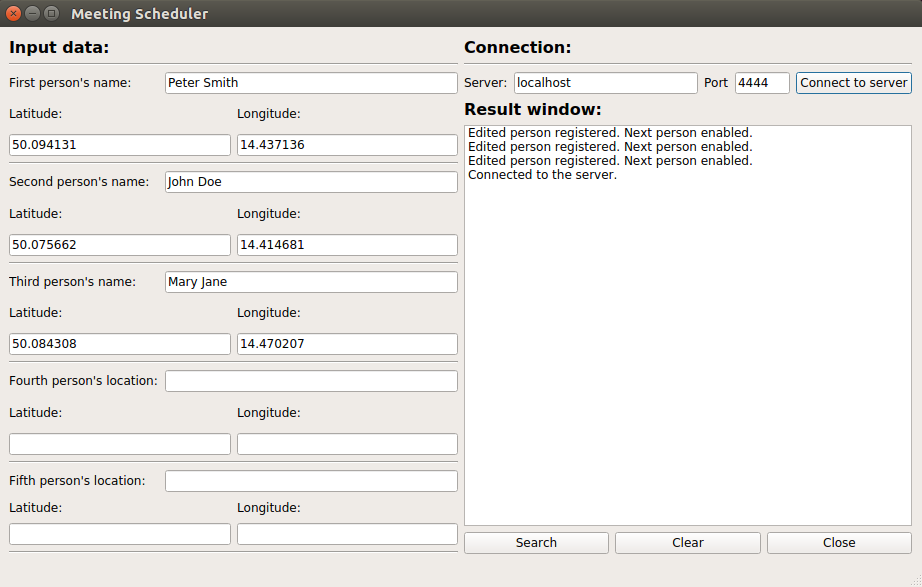
\includegraphics[width=1\textwidth]{pics/UIFinal}
\caption{User interface of the application}
\label{pic:UIFinal}
\end{figure}

The client is split into left and right section. Left section enables the user to enter the locations of people. The edit blocks for other people are uneditable until every person before contains a valid input. For example, after entering the location and the name of the first person, the fields for the second person become editable. After entering proper data into each person's fields, the user is notified in the \textit{Result window} that the next person is available. 

The input required for the application is only a set of latitudes and longitudes in order to locate the position of the person and further use the locations to find a node in the graph and ultimately the optimal meeting point. However, the user interface allows the user to enter the name of the person. This enhances the general user flow, providing the user to associate the location of the coordinates with the name.

In the right section of the client the \textit{Result window} and \textit{Connection} is located. After every action user makes, the \textit{Result window} updates according to the current state of the client or server.

\textit{Connection} allows the user to connect to the server using server address and port. The server and client are connected via transmission control protocol (TCP) as explained in the beginning of the Section \ref{sec:server}. After setting up the connection with the server it is possible to begin the algorithm by pressing \textit{Search} button. Result is afterwards displayed in the \textit{Result window}. Button \textit{Clear} erases all the message in the \textit{Result window}. At last, button \textit{Close} naturally closes the application.


Implemented client is not far of fully optimal user interface mentioned in Section \ref{sec:UIDesign} and meets all the requirements of the sub-optimal version of the UI. 


\chapter{Results}
\label{ch:Results}

For testing the data set of city Prague, capital of Czech republic, was chosen. The data set is available in two versions. First version consist of all the transport nodes available within the area. 
The data set is displayed with QGIS Desktop software on Figure \ref{pic:dataset1}.
\begin{figure}[H]
\centering
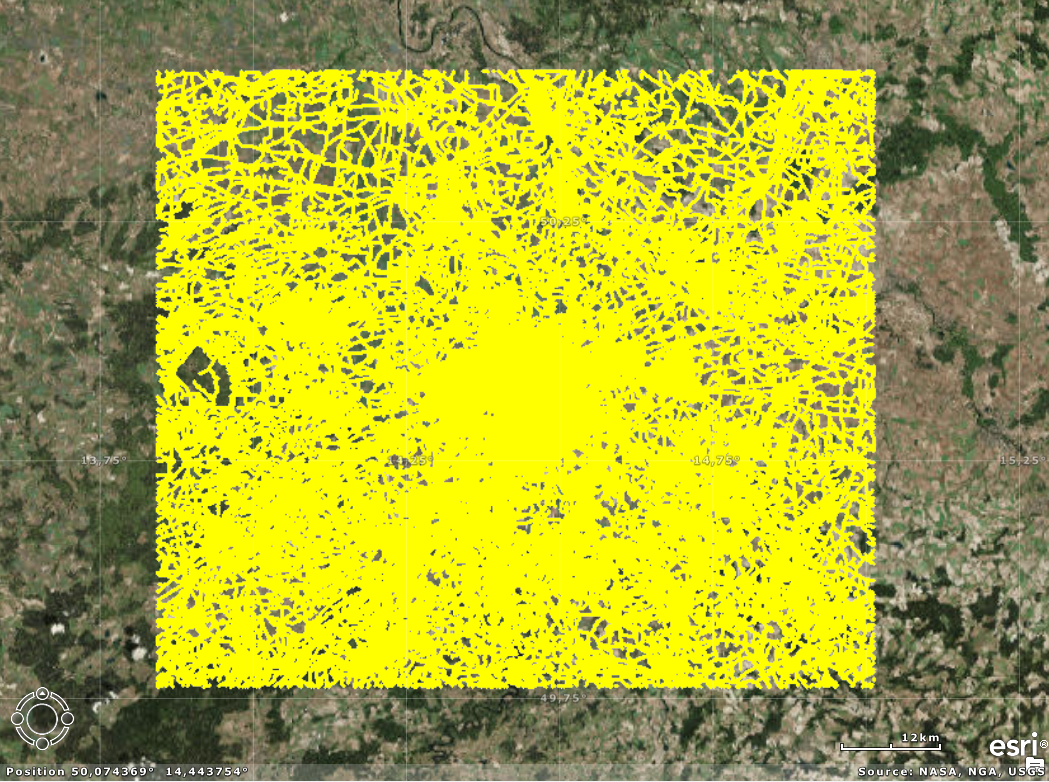
\includegraphics[width=1\textwidth]{pics/praguedatasetL}
\caption{Data set containing the tranportation nodes in the Prague region}
\label{pic:dataset1}
\end{figure}

The second version has a reduced number of nodes using the node reduction technique (see Section \ref{sec:NodeReduction}) with a tolerance of 200 meters. After every 200 meters, one connecting node is being removed.
The second data set is also displayed with QGIS Desktop software on the Figure \ref{pic:dataset2}.
\begin{figure}[H]
\centering
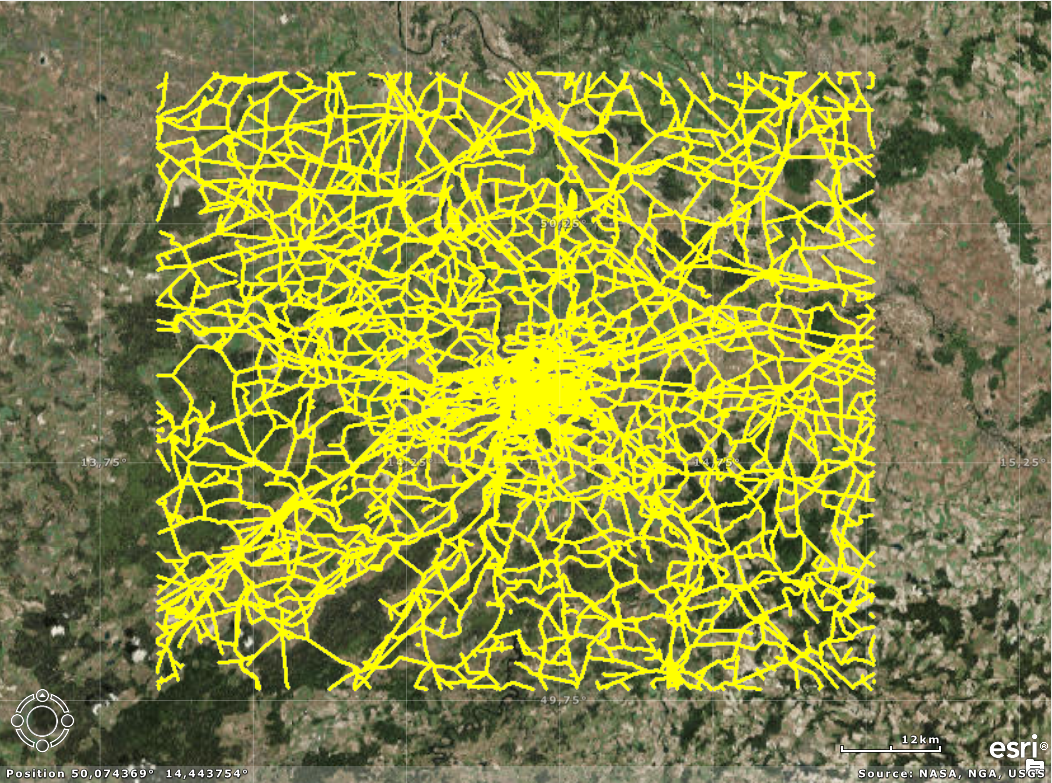
\includegraphics[width=1\textwidth]{pics/praguedatasetS}
\caption{Generalized version of the main Prague data set (reduced number of nodes)}
\label{pic:dataset2}
\end{figure}

The second preprocessing technique described in the Section \ref{sec:Clustering} -- clustering method -- was not used in order to better measure the differences between sequential and parallel solution for the given problem. 

\section{Speed}

\section{Preciseness}

\setsecnumdepth{part}
\chapter{Conclusion}

\section{Future Work}


\bibliographystyle{iso690}
\bibliography{mybibliographyfile}

\setsecnumdepth{all}
\appendix

\chapter{Acronyms}
% \printglossaries
\begin{description}
	\item[APSP] All-pair shortest path
	\item[CERCO] Comit{\' e}e Europ{\' e}en des Responsables de la Cartographie Officielle
	\item[DEM] Digital Elevation Model
	\item[ERDF] European Regional Development Fund
	\item[ESPON] European Observation Network for Territorial Development and Cohesion
	\item[FOSS] Free and Open-Source Software
	\item[GDAL] Geospatial Data Abstraction Library
	\item[GIS] Geographic information systems	
	\item[GUI] Graphical user interface
	\item[MEGRIN] Multi-purpose European Ground Related Information Network
	\item[OOP] Object Oriented Programming
	\item[OSM] OpenStreetMaps
	\item[SSSP] Single-source shortest path
	\item[TCP] Transmission Client Protocol
	\item[XML] Extensible markup language
	
	
\end{description}

\chapter{GDAL/OGR diagram}


\begin{figure}[H]
\centering
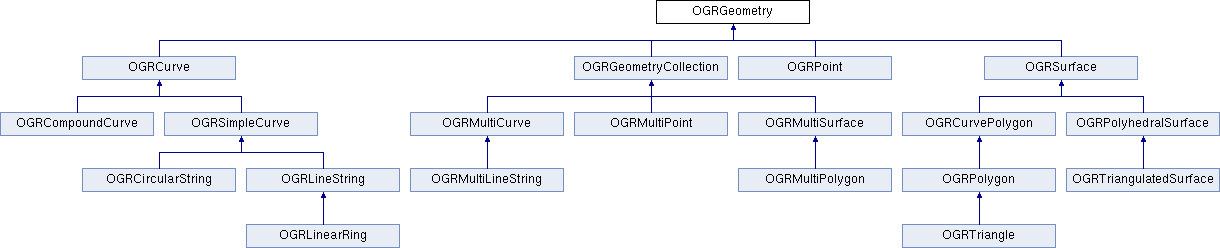
\includegraphics[width=1\textwidth]{pics/classOGRGeometry}
\caption{Inheritance diagram for OGRGeometry}
\label{pic:OGRGeo}
\end{figure}


\chapter{Contents of enclosed CD}

%change appropriately

\begin{figure}
	\dirtree{%
		.1 readme.txt\DTcomment{the file with CD contents description}.
		.1 src\DTcomment{the directory of source codes}.
		.2 server\DTcomment{folder containing server sources}.
		.3 graph\DTcomment{folder containing graph sources}.
		.3 node\DTcomment{folder containing node sources used by graph}.
		.3 data\_reader\DTcomment{folder containing data reading sources}.
		.3 dijkstra\DTcomment{folder containing sources of Dijsktra algorithm}.
		.2 client\DTcomment{folder containing client sources}.
		.2 thesis\DTcomment{the directory of \LaTeX{} source codes of the thesis}.
		.1 text\DTcomment{the thesis text directory}.
		.2 thesis.pdf\DTcomment{the thesis text in PDF format}.
		.2 thesis.ps\DTcomment{the thesis text in PS format}.
	}
\end{figure}

\end{document}
